\chapter{Pipelining the multiplier}
\section{Pipelining}

\section{Fine grain pipelining}
In order to further boost the performance of this floating point multiplier, an additional pipeline register has been inserted in the second stage just after the multiplier. In this case, however, it has been explicitly coded instead of relying of the automatic retiming
\begin{table}
	
	\begin{tabular}{|l|l|l|l|l|}
	\hline
	&\texttt{NPIPE=1} & \texttt{NPIPE=2} & \texttt{NPIPE=4} & \texttt{NPIPE=6}\\\hline
	Delay & 0.78 & 0.71 & 0.68 & 0.72 \\\hline
	Area (total) & & & & \\\hline
	Area (combinational) & & & & \\\hline
	\end{tabular}

	\caption{Critical path delay and area with the hardcoded register in the second stage and a varying \texttt{NPIPE}}
	\label{tab:stage2}
\end{table}

\paragraph{Critical path delay distribution}
\autoref{fig:hist2} and \autoref{fig:hist6} show how worst path delays tend to accumulate towards the shortest one as the degree of pipelining increases. This is a general pattern seen when applying this technique.
\begin{figure}[h]
	\begin{subfigure}{0.5\textwidth}
		\centering
	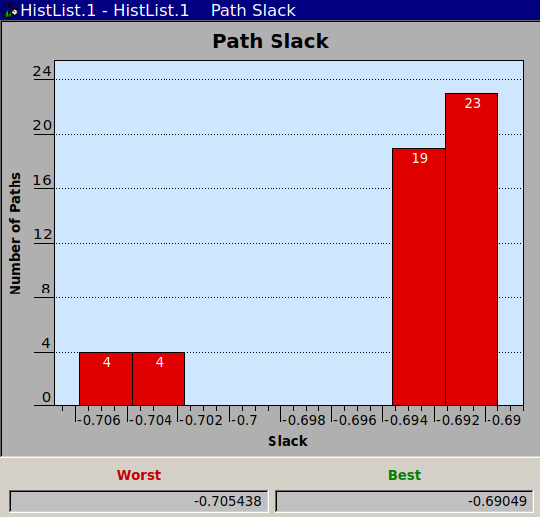
\includegraphics[width=\textwidth]{chapter1/images/npipe2.png}
	\caption{Worst path distribution with \texttt{NPIPE=2}}
	\label{fig:hist2}
\end{subfigure}
\begin{subfigure}{0.5\textwidth}
	\centering
	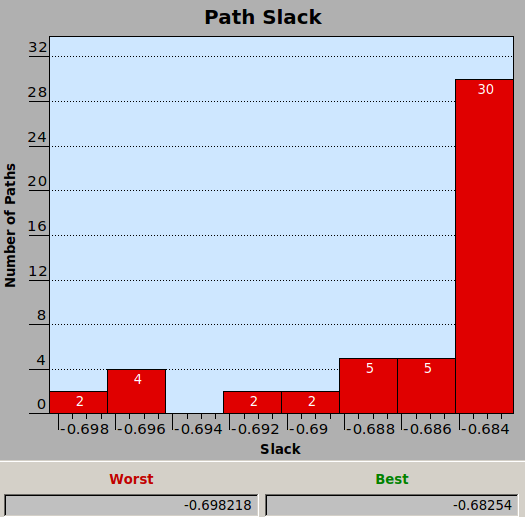
\includegraphics[width=\textwidth]{chapter1/images/npipe6.png}
	\caption{Worst path distribution with \texttt{NPIPE=6}}
	\label{fig:hist6}
	\end{subfigure}
\end{figure}